\documentclass[11pt,a4paper]{article}

% ---------------------------------------------------------------- packages
\usepackage[utf8]{inputenc}
\usepackage[T1]{fontenc}
\usepackage{lmodern}
\usepackage[margin=2.5cm]{geometry}
\usepackage{amsmath,amssymb}
\usepackage{booktabs}
\usepackage{graphicx}
\usepackage{xcolor}
\usepackage{listings}
\usepackage{tikz}
\usetikzlibrary{positioning,arrows.meta,shapes.geometric,fit,calc}
\usepackage{hyperref}
\hypersetup{colorlinks=true,linkcolor=blue!50!black,urlcolor=blue!50!black,citecolor=blue!50!black}

% ---------------------------------------------------------------- listings
\lstdefinestyle{py}{
  language=Python,
  basicstyle=\ttfamily\footnotesize,
  keywordstyle=\color{blue!60!black}\bfseries,
  commentstyle=\color{green!40!black}\itshape,
  stringstyle=\color{red!55!black},
  showstringspaces=false,
  breaklines=true,
  breakatwhitespace=false,
  columns=fullflexible,
  keepspaces=true,
  frame=single,
  rulecolor=\color{black!25},
  backgroundcolor=\color{black!3},
  xleftmargin=4pt, xrightmargin=4pt,
  aboveskip=8pt, belowskip=8pt,
  extendedchars=true,
  inputencoding=utf8,
  literate=
    {→}{{$\rightarrow$}}1 {←}{{$\leftarrow$}}1 {×}{{$\times$}}1
    {≥}{{$\geq$}}1 {≤}{{$\leq$}}1 {≠}{{$\neq$}}1
    {é}{{\'e}}1 {è}{{\`e}}1 {ö}{{\"o}}1 {ü}{{\"u}}1
    {–}{{--}}1 {—}{{---}}1 {…}{{\ldots}}1
    {‘}{{`}}1 {’}{{'}}1 {“}{{``}}1 {”}{{''}}1
}
\lstdefinestyle{yaml}{
  style=py, language={}, keywordstyle={}, stringstyle={},
  morecomment=[l]{\#}, commentstyle=\color{green!40!black}\itshape
}
\lstset{style=py}

\makeatletter
% let long identifiers break after underscores (text mode only)
\DeclareRobustCommand{\_}{\ifmmode\nfss@text{\textunderscore}\else\textunderscore\allowbreak\fi}
\makeatother
\sloppy
\newcommand{\file}[1]{\texttt{#1}}
\newcommand{\NEI}{\textup{NEI}}
\DeclareMathOperator*{\argmax}{arg\,max}

\title{ClaimScan: Architecture and Codebase\\[4pt]
\large A FEVER fact-checker with hybrid retrieval, reranking, rule-based evidence scoring and an NLI verifier}
\author{Generated from the \texttt{ship} branch of \texttt{FEVER\_RAG\_LLM\_Model}}
\date{26 November 2026}

\begin{document}
\maketitle

\begin{abstract}
\noindent
ClaimScan checks a short factual claim against the 25.2 million Wikipedia sentences of the FEVER corpus.
For each claim it retrieves candidate sentences with a hybrid of dense (FAISS, \texttt{bge-small}) and sparse
(BM25, Lucene) search fused by reciprocal rank fusion. A hosted Cohere reranker reorders them, and a small
rule layer rescores them. The best three sentences go to an off-the-shelf DeBERTa-v3 NLI model, whose softmax
output gives the label TRUE, FALSE or NOT ENOUGH INFO (\NEI). Two thresholds turn uncertain verdicts into \NEI.
An optional LLM ``rear aggregator'' can then explain the verdict. The same decision function serves a FastAPI
endpoint and the FEVER benchmark, so the reported numbers describe what the API returns. This document walks through
the code as it is on the \texttt{ship} branch: what each module does, the maths it implements, and how it is
tested, served and evaluated.
\end{abstract}

\tableofcontents
\newpage

% =====================================================================
\section{Overview}
% =====================================================================

The package is \file{claimscan/}. One claim goes through the steps below. They are all run by one function,
\file{pipeline.fact\_check\_detailed}, which the API (\file{api/main.py}), the FEVER evaluation
(\file{eval/fever\_eval.py}) and the FEVER claim test suite all call:

\begin{enumerate}
  \item \textbf{Hybrid retrieval} (\file{retrieval/hybrid\_retriever.py}): FAISS and BM25 each return their top 100
        sentences; reciprocal rank fusion merges them into one ranked list of 100 \texttt{Page\#line} hits.
  \item \textbf{Reranking} (\file{rerank/cohere.py}): Cohere Rerank v3.5 scores the 100 candidates against the claim
        and keeps the top 10. If the call fails, the pipeline keeps the retriever's order.
  \item \textbf{Evidence scoring} (\file{neurosymbolic\_layer/}): every remaining sentence gets a score, a rank prior
        times a product of keyword rules.
  \item \textbf{Evidence selection} (\file{evidence/select.py}): the three best sentences, at most two per page.
  \item \textbf{Verification} (\file{verifier/hf\_nli.py}): \texttt{MoritzLaurer/\allowbreak DeBERTa-v3-base-\allowbreak mnli-fever-anli}
        reads (evidence, claim) as an NLI pair and returns a distribution over TRUE/FALSE/\NEI.
  \item \textbf{\NEI\ rule} (\file{pipeline.py}): a TRUE/FALSE verdict becomes \NEI\ if the top probability is below 0.5
        or $P(\NEI)\ge 0.2$.
  \item \textbf{Rear aggregator} (\file{aggregation.py}, \file{instruct/}): an optional LLM writes an explanation.
        Its veto power is switched off.
  \item \textbf{API} (\file{api/}): FastAPI returns the label, the probabilities, the evidence and the explanation.
\end{enumerate}

Sentence texts come from one read-only SQLite file, never from an in-memory corpus. Figure~\ref{fig:pipeline} shows the whole flow.

\begin{figure}[ht]
\centering
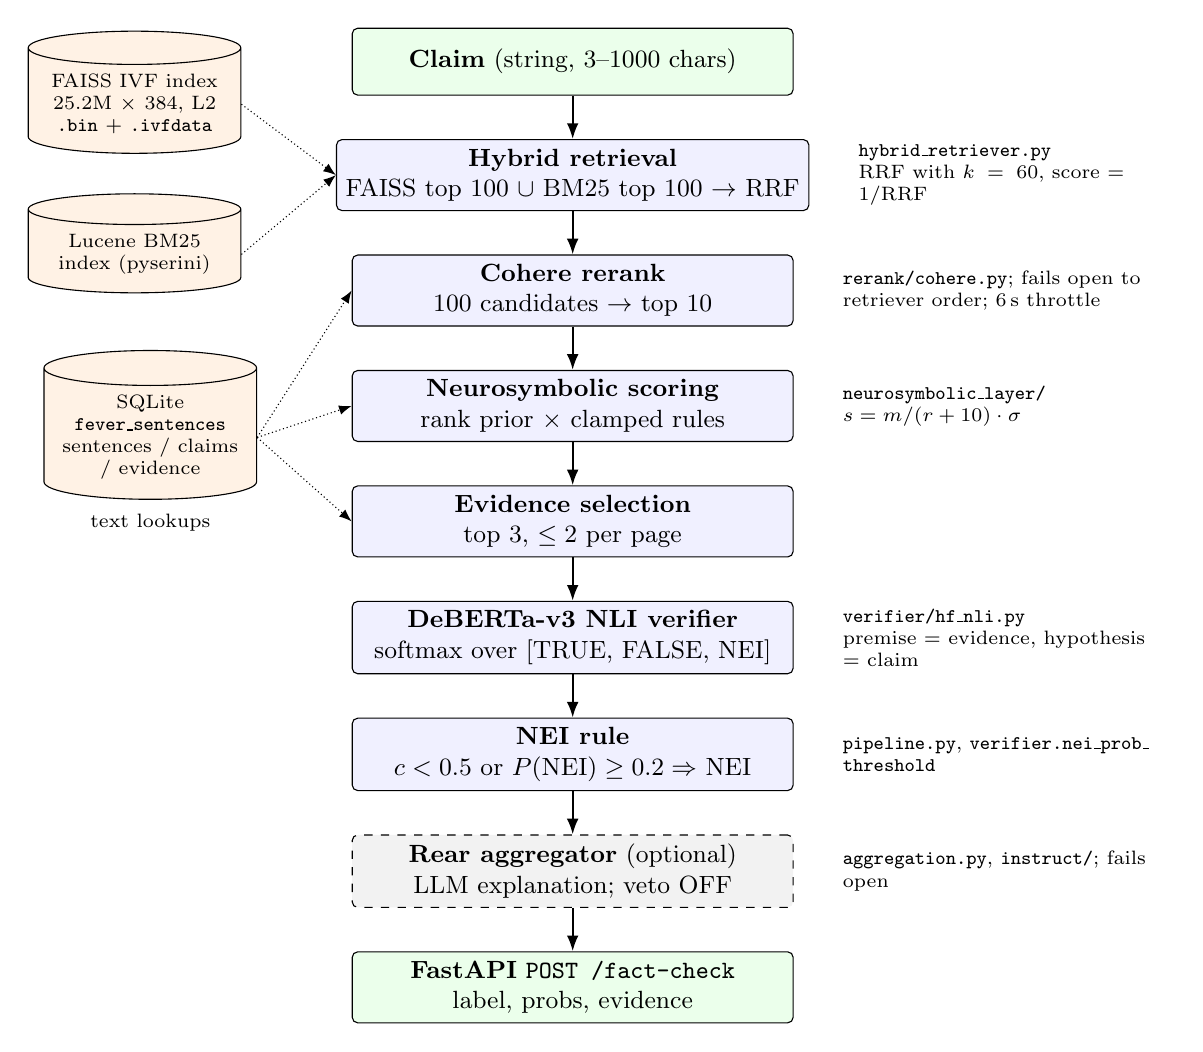
\begin{tikzpicture}[
  node distance=5.5mm,
  stage/.style={draw, rounded corners=2pt, fill=blue!6, minimum width=5.6cm, minimum height=8.5mm,
                align=center, font=\small},
  off/.style={stage, fill=black!5, dashed},
  store/.style={draw, cylinder, shape border rotate=90, aspect=0.18, fill=orange!10, minimum width=2.7cm,
                minimum height=10mm, align=center, font=\scriptsize},
  note/.style={font=\scriptsize, align=left, text width=3.9cm},
  arr/.style={-{Latex[length=2mm]}, thick},
  darr/.style={-{Latex[length=1.6mm]}, densely dotted}
]
\node[stage, fill=green!8] (claim) {\textbf{Claim} (string, 3--1000 chars)};
\node[stage, below=of claim] (hyb) {\textbf{Hybrid retrieval}\\FAISS top 100 $\cup$ BM25 top 100 $\to$ RRF};
\node[stage, below=of hyb] (rr) {\textbf{Cohere rerank}\\100 candidates $\to$ top 10};
\node[stage, below=of rr] (ns) {\textbf{Neurosymbolic scoring}\\rank prior $\times$ clamped rules};
\node[stage, below=of ns] (sel) {\textbf{Evidence selection}\\top 3, $\le 2$ per page};
\node[stage, below=of sel] (ver) {\textbf{DeBERTa-v3 NLI verifier}\\softmax over [TRUE, FALSE, NEI]};
\node[stage, below=of ver] (nei) {\textbf{NEI rule}\\$c<0.5$ or $P(\mathrm{NEI})\ge0.2 \Rightarrow$ NEI};
\node[off, below=of nei] (agg) {\textbf{Rear aggregator} (optional)\\LLM explanation; veto OFF};
\node[stage, fill=green!8, below=of agg] (api) {\textbf{FastAPI} \texttt{POST /fact-check}\\label, probs, evidence};

\foreach \a/\b in {claim/hyb, hyb/rr, rr/ns, ns/sel, sel/ver, ver/nei, nei/agg, agg/api}
  \draw[arr] (\a) -- (\b);

% stores on the left
\node[store, left=12mm of hyb, yshift=9mm] (faiss) {FAISS IVF index\\25.2M $\times$ 384, L2\\\texttt{.bin} + \texttt{.ivfdata}};
\node[store, below=5mm of faiss] (lucene) {Lucene BM25\\index (pyserini)};
\node[store, left=12mm of ns, yshift=-4mm] (sql) {SQLite\\\texttt{fever\_sentences}\\sentences / claims\\/ evidence};
\node[font=\scriptsize, below=0.5mm of sql] {text lookups};
\draw[darr] (faiss.east) -- (hyb.west);
\draw[darr] (lucene.east) -- (hyb.west);
\draw[darr] (sql.east) -- (rr.west);
\draw[darr] (sql.east) -- (ns.west);
\draw[darr] (sql.east) -- (sel.west);

% notes on the right
\node[note, right=5mm of hyb] {\file{hybrid\_retriever.py}\\RRF with $k=60$, score $=1/\mathrm{RRF}$};
\node[note, right=5mm of rr] {\file{rerank/cohere.py}; fails open to retriever order; 6\,s throttle};
\node[note, right=5mm of ns] {\file{neurosymbolic\_layer/}\\$s = m/(r+10)\cdot\sigma$};
\node[note, right=5mm of ver] {\file{verifier/hf\_nli.py}\\premise = evidence, hypothesis = claim};
\node[note, right=5mm of nei] {\file{pipeline.py}, \texttt{verifier.nei\_prob\_threshold}};
\node[note, right=5mm of agg] {\file{aggregation.py}, \file{instruct/}; fails open};
\end{tikzpicture}
\caption{The per-claim pipeline as implemented by \texttt{pipeline.fact\_check\_detailed} and the API. Solid arrows
carry hits and verdicts; dotted arrows are lookups in on-disk stores. The dashed stage is off by default.}
\label{fig:pipeline}
\end{figure}

\paragraph{Services.} \file{pipeline.load\_services} builds a \texttt{Services} dataclass that holds the verifier, the
retriever, a \texttt{SentenceStore} (in the field still called \texttt{corpus\_df}) and an optional reranker. Each is
picked by configuration (\S\ref{sec:config}). Heavy libraries (FAISS, pyserini, sentence-transformers,
LangChain) are imported inside the loader functions, so the verifier and the API can be imported without them.

\paragraph{The decision function.} The core of \file{pipeline.py}, shortened (the returned \texttt{Verdict} also
carries every retrieved hit with its rank, docid, score and text):

\begin{lstlisting}
def fact_check_detailed(claim, services, k=30, conf_threshold=0.5) -> Verdict:
  reranker = getattr(services, "reranker", None)
  evidence_results = services.retriever.search(
      claim, k=config.rerank_candidates if reranker else k)     # 100 with a reranker
  corpus = services.corpus_df
  if hasattr(corpus, "for_hits"):                                # SentenceStore
    corpus = corpus.for_hits(evidence_results)
  if reranker is not None:
    evidence_results = _rerank(reranker, claim, evidence_results, corpus, k)
  picked = get_evidence(claim, evidence_results, corpus, with_ids=True)
  evidence = [text for text, _ in picked]
  if not evidence:
    return Verdict("NOT ENOUGH INFO", 0.0, None, [], hits=hits)
  prediction, probs = verify(services.model, claim, evidence)
  confidence = torch.max(probs).item()
  downgraded = confidence < conf_threshold and prediction != "NOT ENOUGH INFO"
  nei_cut = config.verifier_nei_prob_threshold
  if nei_cut is not None and prediction != "NOT ENOUGH INFO" and probs[2].item() >= nei_cut:
    downgraded = True
  if downgraded:
    prediction = "NOT ENOUGH INFO"
  return Verdict(prediction, confidence, {...}, picked, downgraded, hits=hits)
\end{lstlisting}

\texttt{fact\_check\_cleaned} is a thin wrapper that returns only the label, or the label and the \texttt{Page\#line}
ids of the evidence. The evaluation uses it. The older \texttt{fact\_check} (retrieve 30, no reranker, debug prints)
is kept for the demo script.

% =====================================================================
\section{Data store}
% =====================================================================

\subsection{One SQLite file: \file{claimscan/data/fever\_db.py}}

All FEVER data lives in one SQLite file, \file{<artifacts>/data/processed/fever\_sentences.sqlite}
(\texttt{config.sentence\_store}). It has three tables:

\begin{center}
\begin{tabular}{@{}p{1.9cm}p{7.6cm}p{5.6cm}@{}}
\toprule
Table & Columns & Contents \\
\midrule
\texttt{sentences} & \texttt{id, line, text}; PK \texttt{(id, line)}, \texttt{WITHOUT ROWID} & 25.2M Wikipedia sentences \\
\texttt{claims}    & \texttt{id, split, claim, label}; index on \texttt{id} & 155k claims (train / validation / test) \\
\texttt{evidence}  & \texttt{claim\_id, set\_id, page, line}; index on \texttt{claim\_id} & gold evidence, one row per sentence \\
\bottomrule
\end{tabular}
\end{center}

The builders:
\begin{itemize}
  \item \texttt{download\_claims\_and\_evidence} downloads FEVER v1.0 (\texttt{train}, \texttt{labelled\_dev},
        \texttt{paper\_test}) as parquet from the HuggingFace hub. The HF data has one row per evidence sentence, so a
        claim repeats. The builder normalises claim text, maps labels \texttt{SUPPORTS}$\to$TRUE,
        \texttt{REFUTES}$\to$FALSE, and keeps each claim once (train wins over dev and test). An evidence set is the
        group of rows that share \texttt{set\_id} (the HF \texttt{evidence\_annotation\_id}). \NEI\ claims have no
        evidence rows.
  \item \texttt{build\_sentences(wiki\_zip)} streams the FEVER \texttt{wiki-pages.zip}. Each JSONL page holds
        \texttt{lines} of the form \texttt{num\textbackslash ttext\textbackslash tlinks...}. The builder writes
        \texttt{(page, num, normalize\_text(text))} with \texttt{INSERT OR IGNORE}, skipping a malformed page whole.
\end{itemize}

\texttt{normalize\_text} is the same cleaning that the indexes were built with: Unicode NFKC, lower case, and runs of
whitespace collapsed to one space.

\paragraph{The line-0 fix.} The HF loader wrote sentence 0 of a page as $-1$, which affected 46\% of gold pairs. The
builder writes it back as 0 (\texttt{.replace(-1, 0)}), and \file{eval/gold.py} keeps a \texttt{fix\_line} guard for
old values. The old self-trained verifier (\texttt{deberta\_v1}) was trained on data from before this fix.

\paragraph{Readers.} \texttt{claims(split)}, \texttt{evidence()}, \texttt{sentences(pages)} (queried in chunks of
900 pages to stay under SQLite's parameter limit) and \texttt{iter\_sentences(batch)}, which streams the whole table in
100k-row DataFrames. Read connections open with \texttt{mode=ro}.

\subsection{Serving lookups: \file{claimscan/evidence/store.py}}

\texttt{SentenceStore} is what the pipeline, the API and the evaluation use instead of a 4\,GB pandas corpus.
It opens the file as \texttt{file:...?mode=ro\&immutable=1} with \texttt{check\_same\_thread=False}. The file is
immutable, so SQLite takes no locks, the connection can be shared across the API's worker threads, and the file
can be mounted read-only into a container.

\begin{lstlisting}
def for_hits(self, hits) -> pd.DataFrame:
  keys = list(dict.fromkeys((h["id"], int(h["line"])) for h in hits))   # dedupe, keep order
  rows = []
  for page, line in keys:
    r = self.con.execute("SELECT text FROM sentences WHERE id = ? AND line = ?",
                         (page, line)).fetchone()
    if r is not None:
      rows.append((page, line, r[0]))
  df = pd.DataFrame(rows, columns=["id", "line", "text"])
  return df.set_index(["id", "line"]).sort_index()
\end{lstlisting}

\texttt{for\_hits} returns a frame indexed by \texttt{(id, line)}, the same shape as \texttt{evidence.select.index\_corpus},
so the downstream code is unchanged. Each lookup is a primary-key probe: milliseconds and almost no RAM.
\texttt{lookup(page, line)} returns one text, and \texttt{count()} the row count.

% =====================================================================
\section{Retrieval}
% =====================================================================

Every retriever has the same interface: \texttt{search(query, k)} returns a best-first list of dictionaries
\texttt{\{"id": page, "line": int, "score": float\}}. The FEVER docid \texttt{Page\#line} is split on its last
\texttt{\#} (a line that is not a number becomes $-1$). \file{pipeline.load\_retriever} builds \texttt{faiss},
\texttt{bm25} or \texttt{hybrid} from \texttt{retriever.kind}. The shipped default is \texttt{hybrid}.

\subsection{Dense retrieval: FAISS IVF over \texttt{bge-small}}

\paragraph{Embedding and index build.} \file{retrieval/faiss\_embeddings.py} encodes every sentence as
\texttt{"passage: "+text} with \texttt{BAAI/bge-small-en-v1.5} ($d=384$, L2-normalised). It writes shards of 100{,}000
vectors (\texttt{embeddings\_shard\_*.npy} plus \texttt{docids\_shard\_*.csv}). \file{faiss\_indexer.py} builds an
\texttt{IndexIVFFlat} with $n_\text{list}=4096$ coarse clusters. It trains k-means on the first $\ge 500{,}000$
vectors and then adds shards in one pass. The original index, \file{faiss\_index\_175.bin}, holds shards 4--174
(17.1M vectors); shards 0--3 were used for training only and never added.

\paragraph{Search.} \file{retrieval/faiss\_retriever.py} encodes the query as \texttt{"query: "+claim} with the same
model and normalisation, and calls \texttt{index.search}. An IVF index finds the $n_\text{probe}=64$ centroids nearest
to the query and scans only those inverted lists. The stored index uses the \textbf{L2} metric, so the returned
\texttt{score} is a squared distance (lower is better):
\[
  \mathrm{score}(q,x) = \lVert q - x\rVert_2^2 = 2 - 2\,q^\top x \qquad (\lVert q\rVert=\lVert x\rVert=1),
\]
which ranks the same as cosine similarity. The index file is opened with flags that depend on its layout:

\begin{lstlisting}
ondisk = index_path.with_suffix(".ivfdata").exists()
ONDISK = faiss.IO_FLAG_ONDISK_SAME_DIR | faiss.IO_FLAG_READ_ONLY
self.index = faiss.read_index(str(index_path),
    ONDISK if ondisk else (faiss.IO_FLAG_MMAP if mmap else 0))
if hasattr(self.index, 'nprobe'):
  self.index.nprobe = nprobe
\end{lstlisting}

The shipped index is \file{faiss\_index\_full.bin}. It is small; the inverted lists live in
\file{faiss\_index\_full.ivfdata} (39\,GB), which FAISS memory-maps itself. \texttt{IO\_FLAG\_ONDISK\_SAME\_DIR}
finds the \texttt{.ivfdata} next to the \texttt{.bin}, because the absolute path stored inside the file differs in
Docker, and \texttt{IO\_FLAG\_READ\_ONLY} allows a read-only mount. (Combining \texttt{IO\_FLAG\_MMAP} with an on-disk
index segfaults, hence the branch.) The docid list, a CSV with one row per vector, is loaded into a Python list and
checked against \texttt{index.ntotal}. For 25.2M ids it is the main RAM cost (about 2.5\,GB). A cold query reads
64 lists through 4\,KB page faults over WSL's \texttt{drvfs}, which takes 30--110\,s. Warm queries are fast.

\subsection{Sparse retrieval: BM25 (pyserini/Lucene)}

\file{retrieval/bm25\_index.py} writes one Lucene document per sentence,
\texttt{\{"id": "Page\#line", "contents": "<title> [SEP] <page\_id> [SEP] <sentence>"\}}. The page title is
repeated as a boost. It then runs \texttt{pyserini.index.lucene} with a 512\,MB memory buffer (the 4\,GB default
overflows a capped JVM heap). The index holds 25{,}246{,}092 documents in 4.3\,GB. \file{bm25\_retriever.py} wraps
\texttt{LuceneSearcher} with $k_1=1.2$, $b=0.4$:
\[
  \mathrm{BM25}(q,d) = \sum_{t\in q} \mathrm{idf}(t)\,
     \frac{f_{t,d}\,(k_1+1)}{f_{t,d} + k_1\left(1-b+b\,\frac{|d|}{\overline{|d|}}\right)} ,
\]
where the score is higher-is-better, the opposite of FAISS. RM3 pseudo-relevance feedback is \textbf{off}
(\texttt{bm25.rm3: false}). On FEVER it was both better (label accuracy 0.543 vs 0.537 and FEVER score 0.377 vs
0.337 at $k=30$, old verifier) and about 17$\times$ faster cold (about 0.43\,s vs 7\,s per query).
\texttt{search\_many} runs a batch on Lucene's own thread pool. The JVM starts only when the class is built.

\subsection{Hybrid: reciprocal rank fusion}

\file{retrieval/hybrid\_retriever.py} asks each retriever for $n=\max(k, \texttt{candidates})$ hits
(\texttt{candidates}$=100$). It fuses the hits on the \texttt{(page, line)} key. With $\mathcal{R}=\{\text{faiss},
\text{bm25}\}$ and $\mathrm{rank}_r(d)$ the 1-based position of sentence $d$ in list $r$:
\[
  \mathrm{RRF}(d)=\sum_{r\in\mathcal{R}:\,d\in L_r} \frac{1}{k+\mathrm{rank}_r(d)}, \qquad k=60,
\]
and each fused hit gets
\[
  \texttt{score}(d) = \frac{1}{\mathrm{RRF}(d)} \quad(\text{lower is better, matching the FAISS L2 convention}).
\]
The list is sorted by $\mathrm{RRF}$ in descending order (Python's stable sort keeps first-seen order on ties) and cut
to $k$. A sentence is counted at most once per retriever. Each hit also keeps \texttt{rrf\_score},
\texttt{faiss\_rank} and \texttt{bm25\_rank} (\texttt{None} if not retrieved), so you can see which retriever found
it.

\begin{lstlisting}
for name, hits in ranked_lists.items():
  for rank, hit in enumerate(hits, start=1):
    key = (hit["id"], hit["line"])
    entry = fused.get(key) or fused.setdefault(key, {..., "rrf_score": 0.0})
    if entry[f"{name}_rank"] is None:          # count a sentence once per retriever
      entry[f"{name}_rank"] = rank
      entry["rrf_score"] += 1.0 / (rrf_k + rank)
out = sorted(fused.values(), key=lambda e: e["rrf_score"], reverse=True)
for e in out:
  e["score"] = 1.0 / e["rrf_score"]
\end{lstlisting}

The score direction matters less than it looks. The later evidence scorer uses each hit's \emph{rank}, not its score
(\S\ref{sec:ns}), so FAISS, BM25 and hybrid all work there unchanged.

\subsection{Offline tools: \file{faiss\_batch.py} and \file{faiss\_extend.py}}

\paragraph{\file{faiss\_batch.py}: list-major batch search.} When an evaluation searches hundreds of claims, per-query
search is dominated by random page faults. \texttt{IVFListScanner} turns the search inside out:
\begin{enumerate}
  \item assign every query to its $n_\text{probe}$ lists with the in-RAM coarse quantizer;
  \item group the queries by list and sort the lists by file offset;
  \item a reader thread reads each needed list once with large sequential \texttt{pread}s (a queue of 8 lists reads
        ahead), and the main thread computes exact squared L2 for all queries assigned to that list and keeps a
        running top-$k$ per query with \texttt{argpartition}.
\end{enumerate}
The results equal \texttt{IndexIVFFlat.search} with the same $n_\text{probe}$; only the order of exact ties can
differ. List offsets come either from the on-disk index's list table (codes, then ids at
\texttt{offset + capacity}$\cdot$\texttt{code\_size}) or, for a memory-mapped single file, from the addresses of the
lists inside FAISS's mapping, found via \file{/proc/self/maps}. \texttt{\_check\_offsets} compares a few ids read
both ways before trusting them. \texttt{DocIds} keeps the docid CSV as a pyarrow string array (about 0.6\,GB instead
of about 5\,GB as a Python list). \texttt{batch\_search} ties these together.

\paragraph{\file{faiss\_extend.py}: adding the missing shards.} This script turns the 17.1M index into the full
25.2M one without retraining and without loading the index into RAM:
\begin{enumerate}
  \item find the contiguous run of shards the old index holds (by matching the first docid and summing shard sizes
        to \texttt{ntotal});
  \item for each block of 10 missing shards, build an empty \texttt{IndexIVFFlat} with a \emph{clone of the same
        trained quantizer} (so distances stay comparable) and \texttt{add\_with\_ids} with ids continuing from
        \texttt{ntotal}, appending the docids to a copy of the old CSV in the same order;
  \item merge the old index and all blocks with \texttt{faiss.contrib.ondisk.merge\_ondisk} into
        \file{faiss\_index\_full.ivfdata}, check the total, and write \file{faiss\_index\_full.bin}.
\end{enumerate}
Peak RAM is about one block (about 1.5\,GB). The old index and docids are left untouched.

% =====================================================================
\section{Reranking}
% =====================================================================

\file{claimscan/rerank/} defines one interface (\file{base.py}):
\texttt{rerank(query, docs, top\_n)} returns \texttt{[(doc\_index, score), ...]}, sorted by score in descending
order. \texttt{load\_reranker} picks a backend from \texttt{rerank.backend}: \texttt{none}, \texttt{cross\_encoder}
(local \texttt{sentence-transformers} CrossEncoder, CPU, \texttt{BAAI/bge-reranker-v2-m3}), \texttt{cohere}
(the default) or \texttt{openai} (any OpenAI-compatible chat endpoint, in pointwise 0--10 or RankGPT-style listwise
mode).

\paragraph{Flow.} With a reranker, the pipeline retrieves $\texttt{rerank.candidates}=100$ hits instead of $k=30$.
\texttt{rerank\_hits} looks up each hit's text in the SQLite store, sends the texts to the backend and returns copies
of the hits in the new order, with a \texttt{rerank\_score} added and the retriever's \texttt{score} unchanged.
The pipeline keeps the top $\min(k, \texttt{rerank.top\_n}) = \min(30, 10) = 10$. Hits whose text is missing cannot
be scored; when \texttt{top\_n} is set they are dropped.

\paragraph{Failing open.} \texttt{pipeline.\_rerank} wraps the call:
\begin{lstlisting}
try:
  return rerank_hits(reranker, claim, hits, corpus, top_n=min(k, config.rerank_top_n))
except Exception as e:
  log.warning("reranker failed, keeping retriever order: %r", e)
  return hits[:k]
\end{lstlisting}
A missing \texttt{COHERE\_API\_KEY}, a network error or an HTTP error therefore gives the first 30 retriever hits,
not a failed request.

\paragraph{Cohere client and throttle.} \file{rerank/cohere.py} posts to \texttt{/v2/rerank} with plain
\texttt{httpx}, the model \texttt{rerank-v3.5} and a bearer key read from the environment (never logged). It rejects
more than 1000 documents. A trial key allows about 10 calls per minute, so the client waits until at least
$\texttt{min\_interval}=6$\,s have passed since its previous call. On HTTP 429 or 5xx it retries up to 3 times with
back-off $\min(2^{a}\cdot 2, 30)$\,s for attempt $a$. Results are sorted by \texttt{relevance\_score} (ties by index).
An \texttt{httpx.MockTransport} and a fake \texttt{sleep} can be injected for tests.

% =====================================================================
\section{The neurosymbolic layer: evidence scoring}\label{sec:ns}
% =====================================================================

\file{claimscan/neurosymbolic\_layer/} rescores every retrieved sentence with a few interpretable rules on top of
the neural ranking. It has three files: \file{text.py} (word helpers), \file{rules.py} (the rules) and
\file{score.py} (the combination).

\paragraph{Word helpers.} Every keyword test is whole-word: \texttt{has\_any(text, phrases)} compiles
\verb!\b(?:p1|p2|...)\b! once and caches it, so \emph{if} no longer matches \emph{life}.
\texttt{content\_words(text)} returns the lower-cased alphanumeric tokens that are not stopwords. Tokens of three
letters or fewer are kept only if capitalised (\emph{UK}, \emph{Fox}) or numeric. \texttt{title\_words(page)} turns a
FEVER page id into words: it drops the parenthesised disambiguator (\texttt{-LRB-...-RRB-}) and other escapes such as
\texttt{-COLON-}, replaces \texttt{\_} with spaces and removes stopwords. For example,
\texttt{Savages\_-LRB-2012\_film-RRB-} gives $\{\text{savages}\}$.

\paragraph{The score.} For a claim $c$, a sentence $e$ on page $p$ at 0-based position $r$ in the (reranked) hit list,
\file{score.py} computes
\[
  s(c,e,r,p) \;=\; \sigma(e)\cdot\frac{m(c,e,p)}{r + C}, \qquad C=\texttt{RANK\_C}=10,
\]
where $1/(r+C)$ is the \emph{rank prior}: rank 0 against rank 10 is a factor of 2, so the rules can reorder
neighbours but not lift a sentence from the bottom of the list to the top. The rule multiplier is clamped:
\[
  m(c,e,p) = \operatorname{clip}\!\Big(h(e)\cdot(1+o)\cdot(1+\tfrac12\,t)\cdot\phi(c,e),\; m_{\min}=0.5,\; m_{\max}=3.0\Big).
\]
With $C_c$ the claim's content words, $W_e$ all lower-cased words of $e$, $T_p$ the title words of $p$, and $W_c$ all
words of the claim:
\begin{align*}
  h(e) &= \underbrace{0.5^{[\,e \ni \text{if, suppose, supposedly, hypothetical(ly), would be}\,]}}_{\text{hypotheticals}}
          \cdot \underbrace{0.75^{[\,e\ni\text{probably, perhaps, maybe, possibly}\,]}}_{\text{hedges}},\\[2pt]
  o &= \frac{\lvert C_c \cap (W_e \cup T_p)\rvert}{\max(\lvert C_c\rvert, 1)}
       \qquad\text{(overlap; the title counts because sentences often say ``He\ldots'')},\\[2pt]
  t &= \begin{cases} \lvert T_p \cap W_c\rvert / \lvert T_p\rvert & T_p\neq\emptyset\\ 0 & \text{otherwise}\end{cases}
       \qquad\text{(page-title bonus: the claim names the page)}.
\end{align*}
$\phi(c,e)$ is the product of the claim-type rules in Table~\ref{tab:rules} (1.0 when none applies). Because of the
clamp, no single keyword can sink or dominate a sentence. Two structural penalties are then applied
\emph{outside} the clamp:
\[
  \sigma(e) = 0.3^{[\,|e|_\text{words}<5\,]}\cdot 0.2^{[\,e \ni \text{``disambiguation'' or ``may refer to''}\,]} .
\]

\begin{table}[ht]
\centering\small
\begin{tabular}{@{}p{4.3cm}p{6.6cm}r@{}}
\toprule
Claim mentions & Evidence mentions & factor \\
\midrule
wrote, author(ed), created, made, directed, produced, discovered, featured
  & written by, authored by, created by, recorded by, directed by, produced by, wrote, author of & 1.5 \\
  & else: featuring, starring & 1.25 \\
  & else: published, edition, adaptation, based on & 0.6 \\
made of, composed of & made/composed/comprised/built of, consists of & 1.25 \\
born, died, lived & born (in), died in, was born, birth & 1.3 \\
a superlative (largest, smallest, tallest, biggest, most, least) & exactly the same superlatives & 1.2 \\
capital, located, country & capital of, located in, country, city & 1.3 \\
current(ly), now & a past-role word (served, worked, former(ly), previously, retired) & 0.6 \\
else: former(ly), past, previous(ly) & a past-role word & 1.3 \\
\bottomrule
\end{tabular}
\caption{Claim-type rules in \texttt{rules.filter\_evidence\_by\_claim\_type}; every rule that fires multiplies into
$\phi$. Both texts are lower-cased first.}
\label{tab:rules}
\end{table}

\begin{lstlisting}
def score_evidence_quality(claim, evidence_text, rank, page=None):
  return structural_penalty(rule_multiplier(claim, evidence_text, page) / (rank + RANK_C),
                            evidence_text)
\end{lstlisting}

% =====================================================================
\section{Evidence selection}
% =====================================================================

\file{evidence/select.py} turns hits into the sentences the verifier reads. \texttt{get\_evidence} walks the hits in
order, looks up each text (\texttt{\_lookup\_text} accepts a \texttt{SentenceStore}, an \texttt{(id, line)}-indexed
frame, or a raw frame as a slow fallback), skips hits with no text, and scores each with $s(c,e,r,p)$ from
\S\ref{sec:ns}. The hit's position $r$ is its index among \emph{all} hits, including skipped ones. Candidates are
sorted by $s$ in descending order and passed through \texttt{\_diverse\_top}:

\begin{lstlisting}
TOP_N, MAX_PER_PAGE = 3, 2
def _diverse_top(candidates, n=TOP_N, max_per_page=MAX_PER_PAGE):
  picked, skipped, per_page = [], [], {}
  for c in candidates:
    if per_page.get(c['page'], 0) < max_per_page:
      picked.append(c); per_page[c['page']] = per_page.get(c['page'], 0) + 1
    else:
      skipped.append(c)
    if len(picked) == n:
      return picked
  return picked + skipped[:n - len(picked)]     # back-fill: never fewer than available
\end{lstlisting}

So the evidence is the best three sentences with at most two from one page, unless there are not enough other pages,
in which case skipped sentences fill the free slots. With \texttt{with\_ids=True} each item is
\texttt{(text, "Page\#line")}. These ids are the predicted evidence for the FEVER metric and the citations for
the API and the aggregator.

% =====================================================================
\section{Verifier}
% =====================================================================

\subsection{The NLI model: \file{verifier/hf\_nli.py}}

The default verifier (\texttt{verifier.inference\_model}) is an off-the-shelf NLI model,
\texttt{MoritzLaurer/\allowbreak DeBERTa-v3-base-mnli-fever-anli}, wrapped by \texttt{HFNLIVerifier}. It has the same interface as
the project's own trained \texttt{FEVERVerifier} (\file{deberta\_verifier.py}, selected with the value
\texttt{"ours"}). NLI takes a pair: the \emph{premise} is the evidence sentences joined by spaces and the
\emph{hypothesis} is the claim, truncated to 512 tokens. The model's labels are reordered into the project's label
order by reading \texttt{config.id2label}:

\begin{lstlisting}
NLI_TO_FEVER = {"entailment": 0, "contradiction": 1, "neutral": 2}   # -> TRUE, FALSE, NEI
id2label = {int(i): l.lower() for i, l in self.nli.config.id2label.items()}
self.order = [next(i for i, l in id2label.items() if NLI_TO_FEVER[l] == j) for j in range(3)]

def encode_text(self, claim, evidence):
  return self.tokenizer(" ".join(evidence), claim, max_length=self.max_length,
                        truncation=True, return_tensors="pt")
def forward(self, input_ids, attention_mask):
  return self.nli(input_ids=input_ids, attention_mask=attention_mask).logits[:, self.order]
\end{lstlisting}

The model is loaded in fp32 and runs on CPU; the GPU is kept for LLM training.
(\texttt{FEVERVerifier} is DeBERTa-v3-base with a linear head on the \texttt{[CLS]} vector, reading
\texttt{"claim [SEP] e1 [SEP] e2 ..."}. It is the older checkpoint \texttt{deberta\_v1}.)

\subsection{Decision rule: \file{pipeline.py}}

\texttt{verify} passes at most three evidence sentences. Let $z\in\mathbb{R}^3$ be the reordered logits. Then
\[
  p = \operatorname{softmax}(z),\quad p_j = \frac{e^{z_j}}{\sum_{i} e^{z_i}}\ \ (j\in\{\text{TRUE},\text{FALSE},\NEI\}),
  \qquad \hat y = \argmax_j p_j,\qquad c = \max_j p_j .
\]
With the confidence cut-off $\tau_c = 0.5$ (\texttt{conf\_threshold}, fixed at 0.5 in the API and the evaluation) and
the \NEI\ cut-off $\tau_N = 0.2$ (\texttt{verifier.nei\_prob\_threshold}; \texttt{null} switches it off), the final
label is
\[
  y^{\ast} =
  \begin{cases}
    \NEI & \text{if no evidence sentence was found}\quad(\text{then } c := 0,\ p\text{ undefined}),\\
    \NEI & \text{if } \hat y \neq \NEI \ \text{and}\ \big(c < \tau_c \ \text{ or }\ p_{\NEI} \ge \tau_N\big),\\
    \hat y & \text{otherwise.}
  \end{cases}
\]
The flag \texttt{downgraded} records the second case. The API returns it as \texttt{low\_confidence}. Because
$p$ sums to 1 over three classes, $c\ge 1/3$ always, and the first threshold only fires when the top two classes
are close. The second rule targets the model's main weakness. On gold-\NEI\ claims the median $P(\NEI)$ was only 0.08,
and most errors were \NEI\ claims called TRUE or FALSE with high confidence. The value 0.2 was chosen on the same
300-claim suite it is reported on (\S\ref{sec:results}), so that number is optimistic.

% =====================================================================
\section{Rear aggregator and post-training}
% =====================================================================

\subsection{Purpose and wiring}

The rear aggregator is an LLM that reads the verifier's verdict, probabilities and top-5 evidence for one claim and
returns a structured \texttt{VetoOutput}:
\texttt{veto} (bool), \texttt{veto\_reason}, \texttt{explanation} (1--3 sentences citing \texttt{[page:line]}) and
\texttt{llm\_confidence}$\in[0,1]$ (the model's confidence that the claim is unfactual). It is \textbf{off by default}
(\texttt{aggregator.enabled: false}), API-only (the benchmark never calls it), and \textbf{fails open}.

\begin{itemize}
  \item \file{instruct/schemas.py}: Pydantic shapes between stages. \texttt{ClaimResult} (claim, label, probs,
        evidence) goes in via \texttt{RearInput}; \texttt{ClaimVerdict} and \texttt{RearOutput} come out.
        \texttt{FrontOutput} is reserved for the not-yet-built front decomposer.
  \item \file{instruct/chat\_clients.py}: \texttt{build\_chat(role)} reads \file{llamacpp/roles.yaml}, follows
        \texttt{shares:}, and returns a LangChain \texttt{ChatOpenAI} at \texttt{http://127.0.0.1:<port>/v1}
        (temperature 0, no retries; a \texttt{base\_url} argument overrides it). The caller uses
        \texttt{with\_structured\_output(VetoOutput, method="json\_schema")}, which llama-server turns into a grammar,
        so the JSON always parses.
  \item \file{instruct/rear\_aggregator.py}: the prompt (\texttt{SYSTEM\_PROMPT} plus one user message listing the claim,
        the verdict with probabilities, and the evidence lines tagged \texttt{[page:line]}), the gate
        \texttt{final\_label}, and \texttt{aggregate}, which calls the LLM once per claim and builds the summary in
        code.
  \item \file{aggregation.py}: the glue to the pipeline. \texttt{build\_llm(cfg)} returns the local llama-server client,
        or Together AI's \texttt{ChatTogether} when \texttt{aggregator.api\_key\_env} names an environment variable (the
        config holds only the variable's \emph{name}). \texttt{to\_claim\_result} converts a \texttt{Verdict}
        (after the \NEI\ rule, so a downgraded verdict can never be brought back). \texttt{aggregate\_verdict} never
        raises: on any error it returns the verifier's label with \texttt{aggregator\_error} set, and key values
        are redacted from the log line. It also rejects any verdict other than the verifier's label or \NEI.
        \texttt{build\_hf\_llm} loads the trained adapter in 4-bit on the GPU for offline evaluation and parses the
        reply with \texttt{parse\_veto}.
\end{itemize}

\subsection{The veto gate (currently off)}

The LLM can only \emph{ask} for a veto. Code decides whether it applies, and a veto can only turn TRUE/FALSE into
\NEI, never flip TRUE and FALSE:
\[
  y_\text{final} =
  \begin{cases}
    \NEI & \text{if } \texttt{VETO\_ENABLED} \wedge \texttt{veto} \wedge y^\ast\neq\NEI \wedge
           \big(c < 0.6 \ \vee\ \texttt{llm\_confidence}\ge 0.9\big),\\
    y^\ast & \text{otherwise.}
  \end{cases}
\]
\begin{lstlisting}
VETO_ENABLED = False   # 2026-11-26: the trained adapter vetoed 122/300 claims, 84 of them correct

def final_label(verifier_label, veto, verifier_conf, llm_conf):
  if VETO_ENABLED and veto and verifier_label != NEI and (verifier_conf < 0.6 or llm_conf >= 0.9):
    return NEI
  return verifier_label
\end{lstlisting}
With \texttt{VETO\_ENABLED = False} the LLM only explains. Its veto request still appears in the API response
(\texttt{veto\_requested}, \texttt{veto\_reason}), and the explanation replaces the template response text. The
gate tests switch the veto back on with the \texttt{veto\_on} fixture.

\subsection{Post-training: \file{instruct/posttraining.py}}

The aggregator model is \texttt{google/gemma-3-4b-it} (the \texttt{hf\_model} of the \texttt{aggregator} role). It is
trained with TRL in two stages on the 6\,GB RTX 2060. The base is loaded in 4-bit NF4 with bf16 compute (Gemma
overflows in fp16) and eager attention. Only LoRA adapters are trained ($r=16$, $\alpha=32$, all linear layers).

\paragraph{Data} (\file{data/posttrain\_store.py}, \file{<artifacts>/data/posttrain/posttrain.sqlite}).
The table \texttt{sft\_examples} holds finished chat examples. The \texttt{agg\_*} sources are the aggregator's exact
prompt (\texttt{build\_messages}) with a target \texttt{VetoOutput}: veto iff the verifier's TRUE/FALSE disagrees with
gold, \texttt{llm\_confidence} $=0.95$ for a veto and $0.05$ otherwise. They come from FEVER train claims run through the
full pipeline, and from VitaminC and SufficientFacts run through the verifier only. The table also has VitaminC,
HoVer and LIAR examples for context. \texttt{load\_sft\_dataset} returns TRL prompt/completion rows (UltraFeedback is
excluded). The table \texttt{dpo\_examples} holds UltraFeedback preference pairs, which \texttt{load\_dpo\_dataset}
returns as prompt/chosen/rejected.

\paragraph{SFT.} \texttt{SFTTrainer}, batch 1 with 8-step gradient accumulation, gradient checkpointing,
\texttt{max\_length} 1024, 400 steps. For prompt/completion data TRL's default loss is the token-level negative
log-likelihood of the completion only:
\[
  \mathcal{L}_\text{SFT}(\theta) = -\,\mathbb{E}_{(x,y)}\sum_{t=1}^{|y|}\log \pi_\theta(y_t\mid x, y_{<t}).
\]

\paragraph{DPO.} \texttt{DPOTrainer} starts from the SFT model (4-bit base plus SFT LoRA). TRL copies the SFT adapter
into a frozen adapter named \texttt{"ref"}, which is the reference policy $\pi_\text{ref}$; the code asserts it exists,
so the reference is the SFT model and not the bare base. The run uses 150 steps with the same batch settings.
\texttt{beta} and \texttt{loss\_type} are not set, so TRL's defaults apply (installed TRL 1.19: $\beta=0.1$, loss
\texttt{"sigmoid"}, learning rate $10^{-6}$). That is the standard DPO objective over preference triples
$(x, y_w, y_l)$:
\[
  \mathcal{L}_\text{DPO}(\theta) = -\,\mathbb{E}_{(x,y_w,y_l)}\left[\log \sigma\!\left(
     \beta\log\frac{\pi_\theta(y_w\mid x)}{\pi_\text{ref}(y_w\mid x)}
   - \beta\log\frac{\pi_\theta(y_l\mid x)}{\pi_\text{ref}(y_l\mid x)}\right)\right].
\]
Note that the DPO pairs are general UltraFeedback alignment data, not aggregator-specific pairs. The measured
effect is in \S\ref{sec:results}: the trained adapter copies its SFT targets (\texttt{llm\_confidence} is always
0.95 or 0.05), which is why the veto is now off.

% =====================================================================
\section{Evaluation}\label{sec:eval}
% =====================================================================

\subsection{Gold data: \file{eval/gold.py}}

\texttt{load\_claims(split)} reads claims from SQLite (aliases: \texttt{val}, \texttt{labelled\_dev}$\to$validation).
\texttt{load\_gold\_pairs} gives $\{$claim id$\to$ ordered unique \texttt{(page, line)}$\}$, and
\texttt{load\_gold\_sets} gives $\{$claim id$\to$ list of evidence sets$\}$, each set a sorted list of
\texttt{Page\#line} ids. Page titles are normalised (NFKC, whitespace$\to$\texttt{\_}) on both sides.

\subsection{The FEVER metric and its adapter}

\file{eval/metrics/fever/fever.py} is the FEVER metric from huggingface/evaluate PR \#710, vendored unchanged and
loaded with \texttt{evaluate.load(<dir>)}, so it works offline and is pinned. \file{eval/fever\_eval.py} adapts the
pipeline to it and adds two conventions of the official scorer. Predicted evidence is compared as
\texttt{Page\#line} ids and only the first five count. A gold-\NEI\ claim gets the evidence sets $[[\,]]$, so a correct
\NEI\ label scores.

For claims $i=1..N$ with gold label $y_i$, predicted label $\hat y_i$, gold evidence sets
$\mathcal{S}_i=\{S_{i1},S_{i2},\ldots\}$ and predicted evidence $\hat E_i$ (the first 5 ids, lower-cased; the
pipeline emits 3):
\begin{align*}
  \text{label accuracy} &= \frac1N\sum_{i=1}^N \mathbb{1}[\hat y_i = y_i],\\
  \text{FEVER score} &= \frac1N\sum_{i=1}^N \mathbb{1}\big[\hat y_i = y_i\big]\cdot
                         \mathbb{1}\big[\exists\,S\in\mathcal{S}_i:\ S\subseteq \hat E_i\big],
\end{align*}
where for \NEI\ $\mathcal{S}_i=\{\emptyset\}$, so the evidence condition always holds. The metric also reports
micro-averaged evidence precision and recall against the union $G_i=\bigcup_{S\in\mathcal{S}_i}S$:
\[
  P_\text{ev}=\frac{\sum_i|G_i\cap\hat E_i|}{\sum_i|\hat E_i|},\qquad
  R_\text{ev}=\frac{\sum_i|G_i\cap\hat E_i|}{\sum_i|G_i|},\qquad
  F_1=\frac{2P_\text{ev}R_\text{ev}}{P_\text{ev}+R_\text{ev}} .
\]
Precision includes evidence predicted for \NEI\ claims, and recall uses the union of alternative sets, so both run
low; label accuracy and the FEVER score are the headline numbers. Per claim, the FEVER term is a 0/1 reward. The
planned RL training is meant to import it from here, so the evaluation and the reward cannot drift apart.

\texttt{evaluate\_pipeline} samples \texttt{max\_claims} validation claims (seed 0), runs
\texttt{fact\_check\_cleaned(k=30, conf\_threshold=0.5)} on each, and scores them.

\subsection{Retriever recall: \file{eval/eval\_retriever.py}}

For each validation claim $q$ in the evaluated set $Q$, with gold pairs $G_q$ (the union of its sets) and retrieved
list $L_q$, the script reports the ``any gold sentence'' recall:
\[
  \mathrm{Recall@}k = \frac{1}{|Q|}\sum_{q\in Q} \mathbb{1}\big[\,G_q \cap L_q[1..k] \neq \emptyset\,\big],
  \qquad k\in\{1,5,10,20,50\}.
\]
By default $Q$ is limited to claims with at least one gold pair whose page is in the FAISS index, so all retrievers
are compared on the same claims (\texttt{-{}-all-claims} drops this filter).

\subsection{The benchmark: \file{eval/benchmark.py}}

The benchmark compares \texttt{faiss}, \texttt{bm25} (RM3), \texttt{bm25\_norm3} (no RM3), \texttt{hybrid} and
\texttt{hybrid\_norm3} (the shipped one) on a balanced sample: $n$ claims, a third per label. TRUE/FALSE claims are
limited to those with a gold set fully inside the FAISS index. Each retriever runs in its own subprocess and caches
its hits; FAISS uses the list-major \texttt{faiss\_batch} search. The hybrids are fused from the cached lists exactly
as \texttt{HybridRetriever} does. On TRUE/FALSE claims, with $L_q^k$ the de-duplicated top $k$ and $\mathcal S_q$ the
gold sets, it reports:
\begin{align*}
  \mathrm{hit@}k &= \mathbb{1}[G_q\cap L_q^k\neq\emptyset], &
  \mathrm{recall\_set@}k &= \mathbb{1}[\exists S\in\mathcal{S}_q: S\subseteq L_q^k],\\
  \mathrm{recall@}k &= \frac{|G_q\cap L_q^k|}{|G_q|}, &
  \mathrm{precision@}k &= \frac{|G_q\cap L_q^k|}{k},\\
  \mathrm{MRR} &= 1/\mathrm{rank}_q\ \ (\text{first gold in top 50}), &
  \mathrm{f1@}k &= \text{harmonic mean of the two above},
\end{align*}
each averaged over claims. \texttt{recall\_set@}$k$ is what the FEVER score needs. The benchmark also runs the full
pipeline on every sampled claim for the FEVER metric, times each stage, and logs everything to MLflow.

\begin{figure}[ht]
\centering
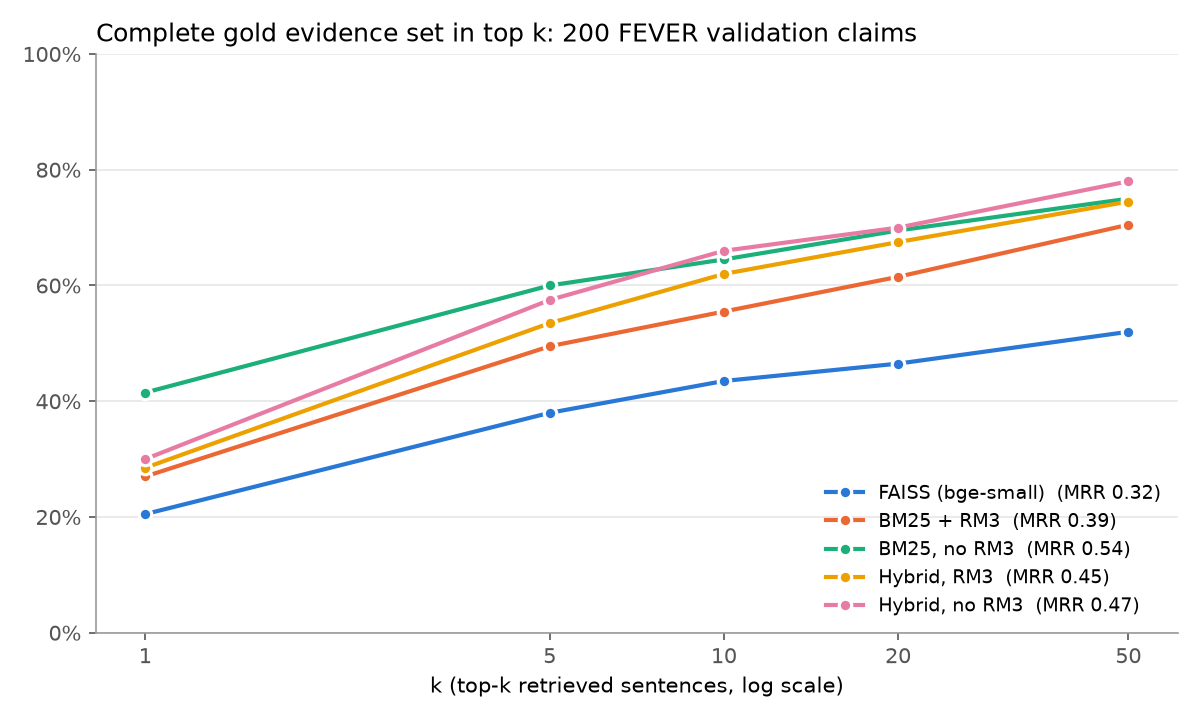
\includegraphics[width=0.82\linewidth]{retriever_recall_set.png}
\caption{\texttt{recall\_set@}$k$ from \texttt{graphs/} (benchmark cache of 2026-11-25: 300 claims, 200 with gold
evidence, on the earlier 17.1M-vector FAISS index, before Cohere reranking). The shipped retriever is ``Hybrid, no
RM3''.}
\label{fig:recall}
\end{figure}

% =====================================================================
\section{API and Docker}
% =====================================================================

\subsection{FastAPI: \file{claimscan/api/}}

\file{api/main.py} defines two routes. The FastAPI lifespan hook loads everything once at start-up
(\texttt{model\_service.load()}: verifier, retriever, sentence store, reranker, and the aggregator if enabled).
\begin{itemize}
  \item \texttt{POST /fact-check} with \texttt{\{"claim": str\}} (3--1000 characters) returns 503 while loading. It
        then runs \texttt{fact\_check\_detailed(claim, services, k=30, conf\_threshold=0.5)}, the same call the
        benchmark makes. Next comes the aggregator if it is on. The response (\texttt{FactCheckResponse},
        \file{api/schemas.py}) has \texttt{prediction}, \texttt{response} text, \texttt{confidence},
        \texttt{probabilities}, \texttt{evidence} (text plus \texttt{Page\#line} source), \texttt{low\_confidence},
        \texttt{latency\_ms}, and, when the aggregator ran, \texttt{verifier\_prediction}, \texttt{veto\_requested},
        \texttt{vetoed}, \texttt{veto\_reason}, \texttt{llm\_confidence}, \texttt{explanation} and
        \texttt{aggregator\_error}. Unexpected errors are logged and returned as a generic 500.
  \item \texttt{GET /health} returns \texttt{\{"status": "healthy", "models\_loaded": bool\}}.
\end{itemize}
The endpoint is a plain \texttt{def}, so FastAPI runs it in a worker thread and \texttt{/health} stays responsive.
A \texttt{threading.Lock} (\file{api/deps.py}) serialises claims, because inference is CPU-bound and the Lucene
searcher is not thread-safe.

\subsection{Docker}

The \file{Dockerfile} builds a CPU-only image on \texttt{python:3.12-slim-trixie}, which has OpenJDK 21 for pyserini.
It installs CPU torch first, so \texttt{requirements.txt} never pulls CUDA wheels, and asserts the build is CPU. It
copies only \file{configs/} and \file{claimscan/} and runs as an unprivileged user with one uvicorn worker.
\texttt{HF\_HUB\_OFFLINE=1}, so nothing is downloaded at run time. A health check reads
\texttt{models\_loaded}, with a 25-minute start period because the indexes are large. \texttt{WITH\_BM25=0} builds a
smaller FAISS-only image.

\file{docker-compose.yml} mounts the data \textbf{read-only}:
\begin{lstlisting}[style=yaml]
volumes:
  - ${CLAIMSCAN_ARTIFACTS_HOST:-/mnt/d/crisis-claim-analysis/artifacts}:/artifacts:ro
  - ${HF_CACHE_HOST:-/mnt/d/huggingface_cache}:/hf:ro
\end{lstlisting}
\texttt{CLAIMSCAN\_ARTIFACTS=/artifacts} makes every configured path resolve inside the mount. Read-only mounts work
because of the read-only design of every loader. FAISS opens the \texttt{.ivfdata} with \texttt{IO\_FLAG\_READ\_ONLY}
and finds it next to the \texttt{.bin}. SQLite opens with \texttt{immutable=1}. Lucene only reads. API keys
(\texttt{COHERE\_API\_KEY}, an optional LLM key) are passed through from the shell or an untracked \file{.env}, never
written to a committed file. An optional \texttt{llama} service (profile \texttt{aggregator}) runs
\texttt{ghcr.io/ggml-org/llama.cpp:server} with the GGUF directory mounted read-only, on host port 8083 (the
aggregator's port in \file{roles.yaml}). The API does not depend on it, because the aggregator fails open.

% =====================================================================
\section{Configuration}\label{sec:config}
% =====================================================================

\file{claimscan/config.py} reads \file{configs/default.yaml} (or the file named by \texttt{CLAIMSCAN\_CONFIG}) into a
\texttt{ClaimScanConfig} dataclass, resolving relative paths against \texttt{artifacts\_root}. Environment variables
override a few values: \texttt{CLAIMSCAN\_ARTIFACTS}, \texttt{CLAIMSCAN\_RETRIEVER} and
\texttt{CLAIMSCAN\_AGGREGATOR\_\{ENABLED, URL, MODEL, TIMEOUT, API\_KEY\_ENV\}}. \texttt{hf\_home} is applied only if
\texttt{HF\_HOME} is unset. The settings that shape behaviour:

\begin{center}\small
\begin{tabular}{@{}p{5.2cm}p{5.0cm}p{4.5cm}@{}}
\toprule
Key & Value & Effect \\
\midrule
\texttt{retriever.kind} & \texttt{hybrid} & FAISS + BM25 with RRF \\
\texttt{retriever.model} & \texttt{BAAI/bge-small-en-v1.5} & query encoder (384-d) \\
\texttt{retriever.index\_file} & \texttt{faiss\_index\_full.bin} & 25.2M vectors, on-disk lists \\
\texttt{retriever.nprobe} & 64 & IVF lists scanned per query (of 4096) \\
\texttt{retriever.mmap} & \texttt{true} & memory-map a single-file index \\
\texttt{bm25.k1}, \texttt{bm25.b}, \texttt{bm25.rm3} & 1.2, 0.4, \texttt{false} & BM25 parameters, no RM3 \\
\texttt{hybrid.rrf\_k}, \texttt{hybrid.candidates} & 60, 100 & RRF constant, hits per retriever \\
\texttt{rerank.backend} & \texttt{cohere} (\texttt{rerank-v3.5}) & reranker \\
\texttt{rerank.candidates}, \texttt{rerank.top\_n} & 100, 10 & reranker input / output size \\
\texttt{verifier.inference\_model} & \texttt{MoritzLaurer/\allowbreak DeBERTa-v3-base-\allowbreak mnli-fever-anli} & verifier \\
\texttt{verifier.nei\_prob\_threshold} & 0.2 & $P(\NEI)\ge\tau_N \Rightarrow$ \NEI \\
\texttt{verifier.max\_length} & 512 & NLI input tokens \\
\texttt{aggregator.enabled} & \texttt{false} & rear aggregator off \\
\texttt{aggregator.api\_key\_env} & \texttt{""} & empty = local llama-server; a name = Together AI \\
\bottomrule
\end{tabular}
\end{center}

The YAML also lists the other dense indexes (\texttt{minilm}, \texttt{e5\_base}) for the embedding and indexing scripts,
and the training settings of the old verifier. The code also fixes some values: $k=30$ and
$\tau_c=0.5$ in the API and evaluation, \texttt{RANK\_C}$=10$ and the clamp $[0.5, 3]$ in the scoring layer, top 3 / max
2 per page in selection, and the veto thresholds 0.6/0.9.

% =====================================================================
\section{llama.cpp roles}
% =====================================================================

\file{llamacpp/roles.yaml} has one entry per LLM role, following the plan's ``one config per LLM role''. A
\texttt{llamacpp} role is a local \texttt{llama-server} at \texttt{127.0.0.1:<port>}; a \texttt{hosted} role uses a base
URL and a key read from a named environment variable.

\begin{center}\small
\begin{tabular}{@{}p{2.5cm}p{5.6cm}p{0.9cm}p{5.1cm}@{}}
\toprule
Role & Model (GGUF, file names still TODO) & Port & Notes \\
\midrule
\texttt{research\_agent} & Qwen3-4B Q4\_K\_M & 8081 & GBNF action grammar; LoRA later \\
\texttt{reranker} & Qwen3-Reranker-0.6B Q8\_0 & 8082 & \texttt{-{}-reranking} \\
\texttt{front\_facer} & Qwen3.5-9B Q4\_K\_M & 8085 & partial GPU offload; thinking off \\
\texttt{decomposer} & shares \texttt{front\_facer} & 8085 & JSON via \texttt{json\_schema} \\
\texttt{aggregator} & Gemma-3-4B-it Q4\_K\_M; HF weights \texttt{google/\allowbreak gemma-3-4b-it} & 8083 & used by the API \\
\bottomrule
\end{tabular}
\end{center}

\paragraph{Status: scaffold.} On \texttt{ship}, only the \texttt{aggregator} role is used by code
(\texttt{chat\_clients.build\_chat} and the training script). The others are configuration for the planned agent.
\file{llamacpp/README.md} is a step-by-step walkthrough (build, models, sanity checks, launch script, Python client).
The \textbf{CUDA build is blocked}: CUDA 12.4's \texttt{nvcc} accepts host gcc $\le 13$, and the WSL system has gcc 15.
The README lists three ways out: a CPU build now, a newer CUDA toolkit (12.8+) installed on E:, or gcc-13 alongside.
\file{scripts/build.sh} targets \texttt{sm\_75} (RTX 2060), and \file{scripts/serve.sh} is a skeleton. The front MoE
model does not fit in 15\,GB of RAM, so those roles are meant to go to a hosted API.

% =====================================================================
\section{Tests and CI}
% =====================================================================

\file{tests/} has 145 test functions in 18 files. They need no GPU and no large artifacts. Models, servers and
networks are stubbed (\texttt{httpx.MockTransport} for Cohere and the OpenAI wire format, fake structured LLMs, tiny
SQLite stores, toy FAISS indexes). The main groups:

\begin{center}\small
\begin{tabular}{@{}p{6.4cm}p{8.6cm}@{}}
\toprule
File(s) & What is pinned \\
\midrule
\texttt{test\_scoring.py} & the neurosymbolic rules, clamp, rank prior, diversity selection \\
\texttt{test\_hybrid\_retriever.py} & RRF maths, tie order, candidates; BM25/Lucene end to end \\
\texttt{test\_rerank.py} & backends, \texttt{rerank\_hits}, Cohere retries and throttle, pipeline use \\
\texttt{test\_store.py}, \texttt{test\_verifier\_data.py} & SQLite store; line-0 fix and data prep \\
\texttt{test\_faiss\_indexer.py}, \texttt{test\_faiss\_extend.py} & index build and search; extending with the missing shards \\
\texttt{test\_benchmark.py} & list-major FAISS scan equals \texttt{index.search}, metrics, MLflow \\
\texttt{test\_fever\_metric.py} & vendored metric, adapter conventions, gold loaders \\
\texttt{test\_rear\_aggregator.py}, \texttt{test\_aggregation.py} & veto gate (with \texttt{veto\_on}), never TRUE$\leftrightarrow$FALSE, fail-open \\
\texttt{test\_aggregator\_llm\_output.py}, \texttt{test\_instruct\_model.py} & real LangChain stack on fake HTTP; roles.yaml clients \\
\texttt{test\_api.py}, \texttt{test\_config.py}, \texttt{test\_imports.py} & endpoint wiring with stub services; config; imports \\
\texttt{test\_posttrain\_store.py} & SFT rows and TRL dataset shapes \\
\texttt{test\_fever\_suite.py} & end-to-end FEVER suite (artifacts; deselected by default) \\
\bottomrule
\end{tabular}
\end{center}

\file{tests/conftest.py} deselects the slow FEVER suite unless its file is named or \texttt{-m fever\_suite} is
given. The suite runs the 300-claim benchmark sample end to end and compares per-claim flips against
\file{tests/data/fever\_suite\_hybrid\_norm3\_baseline.json}. Its gold-evidence measurement runs only with
\texttt{-k gold\_evidence}. \texttt{pytest} runs with \texttt{-{}-capture=sys}, because the default tmpfile capture
fails on WSL's \texttt{drvfs}.

\paragraph{CI.} \file{.github/workflows/unit-tests.yml} runs on every push and pull request (and by hand), and
cancels superseded runs. Ubuntu, Python 3.12 and Temurin Java 21 (for pyserini), CPU torch installed first, then
\texttt{requirements-dev.txt} and the package in editable mode. \texttt{CLAIMSCAN\_ARTIFACTS} points at an empty
directory, so artifact tests skip themselves, and \texttt{HF\_HUB\_OFFLINE=1}, so a test can never download a model.
It runs \texttt{python -m pytest -q -rs}. Accuracy is measured locally, not in CI.

% =====================================================================
\section{Current results and direction}\label{sec:results}
% =====================================================================

All numbers below are from the project notes. They were measured on the 300-claim FEVER validation suite (balanced,
100 claims per label, seed 0), with $k=30$, the full FAISS index, Cohere reranking and the ready-made verifier,
on 2026-11-26.

\begin{center}\small
\begin{tabular}{@{}lccccc@{}}
\toprule
Configuration & Label acc. & FEVER score & TRUE & FALSE & NEI \\
\midrule
Verifier, confidence cut-off only & 0.650 & 0.467 & 91\% & 76\% & 28\% \\
+ NEI rule $\tau_N=0.2$ (\textbf{default}) & 0.670 & -- & 90\% & 72\% & 39\% \\
Gemma DPO aggregator, veto on & 0.463 & 0.373 & & & \\
\midrule
2026-11-25: ready-made verifier & 0.64 & 0.48 & & & \\
2026-11-25: old \texttt{deberta\_v1} & 0.51 & 0.38 & & & \\
\bottomrule
\end{tabular}
\end{center}

\begin{itemize}
  \item \textbf{Errors are mostly \NEI.} 72 of the 105 errors in the 0.65 run were \NEI\ claims called TRUE or FALSE
        (50 of them with confidence $\ge 0.9$). In samples, several of these are actually supported by the retrieved
        sentences, which points to label noise in FEVER's \NEI\ class. The NEI rule recovers part of this. Its
        threshold was chosen on these same 300 claims.
  \item \textbf{Retrieval is not the main limit.} For 131 of the 200 TRUE/FALSE claims the full gold set reached the
        verifier, and the verifier was right on 85\% of those. With gold evidence alone the ready-made verifier
        scores 82\% on the suite's TRUE/FALSE claims (the old one 57\%).
  \item \textbf{The veto hurt.} The DPO-trained aggregator vetoed 122 claims, 84 of which had correct verdicts. Its
        confidence was always 0.95 or 0.05, so the $\ge 0.9$ gate never filtered anything. The veto is now off and the
        LLM only explains.
\end{itemize}

\paragraph{Planned direction.} None of this is built on \texttt{ship} yet. The plan puts a research agent in front
of the verifier: a local Qwen3-4B decomposer on llama.cpp that splits a user's text into atomic claims, writes search
queries, and decides after each round whether to search again or stop. It would run as a per-claim retrieval loop
(retrieve, rerank, verify; at most three hops). This ``librarian'' would be trained with LoRA SFT and then
reinforcement learning (GRPO), with the frozen verifier and the per-claim FEVER score of \S\ref{sec:eval} as the
reward. The plan also names a more structured reasoning layer, natural-logic and first-order-logic checks between
claim and evidence, to go beyond the keyword rules of \S\ref{sec:ns}. Throughout, the \emph{explanation} (which
sentences support or refute which part of the claim) is meant to become the main output rather than a by-product
of the label. A later use of the same machinery is a paper-reading helper: highlight a term and get a grounded
1--2 sentence definition.

\end{document}
